\section{Generative Fitting} \label{sec:generative_fitting}

The generative fitting service is the most demanding procedure in the context of processing resources. The service represents the filtering and compression operations presented in Section \ref{sec:high_level_overview}. There are two scenarios based on the region's complexity. If the region is not complex, no further actions are taken except it formally was complex. Then, existing models have to be deleted, since they are not longer used. And if the region is complex, generative models are provided, which represent the exchange medium for information. More specifically, multiple \textit{Gaussian Mixture Models} (GMMs) are fitted on each label-subset of a region's data, which was stored in the indexing step in Section~\ref{sec:local_indexing}. According to a model selection process that evaluates the efficacy of each GMM, the best model is stored in the global pattern database, accessible to every member in the CIDS. The purpose of that elaborate process is that synthetic data can be sampled from these models. This way, every member has access to the global knowledge from all local infrastructures in order to enhance the local dataset that is used for fitting a classifier. Thus, this service is the key for providing \textit{privacy} and \textit{minimal overhead} while exchanging information.
% WHY GMMs? and not NNs for example?
\begin{algorithm}
    \caption{Retrieve Dataset from Region (Main Procedure)}
    \label{alg:generative_fitting}
    \algsetup{indent=2em}
 
    \begin{algorithmic}[1]
        \REQUIRE Regions $R_{\text{in}}$
        \ENSURE Regions $R_{\text{out}}$

        \STATE $m \leftarrow$ getID()
        \FORALL{$r$ in $R_{\text{in}}$}

            \STATE $k_\kappa \leftarrow \text{concatenate}(p_c, r)$
            \STATE $k_\delta \leftarrow \text{concatenate}(p_y, r, m)$

            \STATE $c_r \leftarrow PDB_G[k_\kappa]$
            \STATE $Y_r \leftarrow PDB_G[k_\delta]$ % get label set of region from global PDB

            \IF{$c_r = 0$}
                \FORALL{$y$ in $Y_r$}
                    \STATE $k_\omega \leftarrow \text{concatenate}(p_d, r, y, m)$ 
                    \STATE delete model in $PDB_G[k_\omega]$
                \ENDFOR
            \ELSE
                \STATE $L \leftarrow$ new List
                \FORALL{$y$ in $Y_r$}
                    \STATE $k_\alpha \leftarrow \text{concatenate}(p_x, r, y)$
                    \STATE $H \leftarrow PDB_{L_m}[k_\alpha]$
                    \STATE append $H$ to $L$
                \ENDFOR

                \STATE $D \leftarrow \text{preprocessing}(L)$

                \FORALL{$y$ in $Y_r$}
                    \STATE $\text{GMM} \leftarrow \text{modelSelection}(D, y)$
                    \STATE $k_\omega \leftarrow \text{concatenate}(p_d, r, y, m)$ 
                    \STATE $PDB_G[k_\omega] \leftarrow \text{GMM}$
                \ENDFOR
            \ENDIF
            


        \ENDFOR
    \end{algorithmic}
 \end{algorithm}

 First, regions that have been updated are received as events. As the data is further organized per label within a region, the labels for a region are retrieved. Then, if the region is not complex, no model fitting is executed. Instead, potentially existing models are deleted from storage. This is the case, if the complexity status of the has been changed from complex to simple.

 But if the region is complex, the generative model fitting procedure is triggered. Even if there are already models for the corresponding combination of region and label, an update of these models is initialized. For that, every hash table within a region, each containing data with a common label, is collected and added to a list. Subsequently, preprocessing operations prepare the collected region data for the model fitting. Details on the data preparation are described in Algorithm \ref{alg:data_preprocessing}.

 After that, the Model Selection process is started sequentially for each available label in the region. That way, the models are only fitted on data with the label in focus but evaluated with the complete region data. Specifics on the model selection are elaborated in Algorithm~\ref{alg:model_selection}. Finally, the best fitted model is stored in the global pattern database. So far, the main procedure has been outlined. Next, the details on the data preprocessing and the model selection are elaborated.

 \begin{algorithm}
    \caption{Preprocess Data}
    \label{alg:data_preprocessing}
    \algsetup{indent=2em}
 
    \begin{algorithmic}[1]
        \REQUIRE List of HashMaps $L$
        \ENSURE Dataset $D$
        
        \STATE $D \leftarrow \text{getValues(L)}$
        \FORALL{label in $D$}
            \IF{label $\neq 0$}
                \STATE \COMMENT{split into binary}
                \STATE $(X_a, y_a) \leftarrow (X, y)$ where $y=\text{label}$ 
                \STATE $(X_b, y_b) \leftarrow (X, y)$ where $y \neq \text{label}$
                \IF{$X.\text{shape}[0] < X.\text{shape}[1]$}
                    \STATE $X_a, y_a \leftarrow \text{upsample}(X_a, y_a)$
                \ENDIF
            \ENDIF
        \ENDFOR
        \RETURN $(X_a, y_a), (X_b, y_b)$
    \end{algorithmic}
 \end{algorithm}

 Starting with the preprocessing.

 Splitting the dataset into a binary problem, such that the label that is currently in focus is the normal class and all other classes are attack classes. That way, the generative model can be evaluated using the machine learning efficacy method in the later course. 

 The upsampling process ensures that the fitting algorithm for the GMM is able to work. In practice, the number of samples has to be at least equal to the number of components. As some label subsets of a region may exhibit a low number of samples, in extreme cases only a single sample, an upsampling process is implemented. In particular, a set of nearest neighbours is generated per sample. First, the number of samples to generate is determined by the difference of the dimensionality of the data and the number of data points. Then, in order to generate from each data point equivalently, the number of nearest neighbours to sample is determined per data points. That is, the complete number of points to resample divided by the number of samples with an interger division (resulting in an integer). In case, the result of the interger division is zero, one is added to the result. Then for each data point $x$ in the set $X$, nearest neighbours are generated by sampling from a uniform distribution. This is done by considering each feature value of $x$ individually, such that the nearest neighbour is the concatenation of the sampled feature values as $x^* = [p(x_1), p(x_2), \dots, p(x_M)]$, where $p(x_m)=\frac{1}{b-a}$ within the interval $[x_m-\delta, x_m+\delta)$. The value $\delta$ controls the interval of the uniform distribution. The larger the value for $\delta$, the further the newly generated values deviate from the orginal feature values. In Figure \ref{subfig:hist_nn} the value for a single feature $x_m$ is drawn uniformly at random. The original value of the feature was $x_m=4$, which was extended by $\delta=1\cdot10^{-2}$. By choosing a relatively small value for $\delta$, it is ensured that the generated nearest neighbours do not alter the original data distribution significantly, while enabling the subsequent fitting of the GMM for that set of data points.


 \begin{figure}%
    \centering%
    \begin{subfigure}[b]{0.49\textwidth}%
        \centering\captionsetup{width=.8\linewidth}%
        % \documentclass{standalone}
% \usepackage{pgfplots}
% \pgfplotsset{compat=1.17}
% \begin{document}
\begin{tikzpicture}[
    declare function={unipdf(\x,\xl,\xu)= (\x>\xl)*(\x<\xu)*1/(\xu-\xl);}
]
\begin{axis}[
    width=6cm,height=6cm,
    axis lines=left,
    scaled y ticks=false,
    xlabel={$x$},
    ylabel={$p(x)$},
    every axis y label/.style={at={(current axis.north west)},above=0mm},
    every axis x label/.style={at={(current axis.south east)},right=0mm},% axis lines=left,
    samples=100,
    const plot mark mid,
    ymin=-0.02,
    ymax=1.15,
    xmin=-0.25,
    xmax=1.25,
    ytick={0, 0.667},
    yticklabels={ $0$, $\frac{1}{b-a}$},
    xtick={0,1},
    xticklabels={$a$, $b$}
]
\addplot [very thick, black!50] {unipdf(1.5*x,0,1.5)};
\end{axis}
\end{tikzpicture}
% \end{document}%
        \caption{The pdf of a uniform distribution is $p(x) = \frac{1}{b-a}$ within the interval $[a, b)$, and zero elsewhere.}%
        \label{subfig:uniform_dist}%
    \end{subfigure}%
    \hfill%
    \begin{subfigure}[b]{0.49\textwidth}%
        \centering\captionsetup{width=.8\linewidth}%
        \documentclass{standalone}
\usepackage{pgfplots}
\pgfplotsset{compat=1.17}
\begin{document}

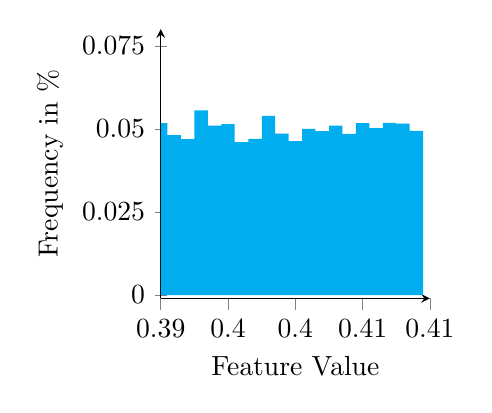
\begin{tikzpicture}

    \begin{axis}[
        width=5cm,height=5cm,
        axis lines=left,
        scaled y ticks=false,
        ylabel={Frequency in \%},
        xlabel={Feature Value},
        legend style={at={(0.5,-0.1)},
        anchor=north,legend columns=-1},
        ybar=0pt,
        bar width=4.8pt,
        ymin=-0.001,
        ymax=0.080,
        ytick={0, 0.025, 0.05, 0.075},
        yticklabels={$0$, $0.025$, $0.05$, $0.075$},
        xmin=0.39,
        xmax=0.41,
        % xtick={0.2, 0.4, 0.6,/ 0.8, 1.0}
    ]
    \addplot[draw opacity=0.0, fill=cyan]
        coordinates {
            (0.3900009, 0.051699999999999996)
            (0.3910007, 0.0481)
            (0.3920006, 0.046900000000000004)
            (0.3930004, 0.0556)
            (0.3940003, 0.051)
            (0.3950001, 0.051399999999999994)
            (0.396, 0.046)
            (0.3969998, 0.047)
            (0.3979997, 0.053899999999999997)
            (0.3989995, 0.048600000000000004)
            (0.3999994, 0.0463)
            (0.4009993, 0.05)
            (0.4019991, 0.0493)
            (0.402999, 0.051)
            (0.4039988, 0.048499999999999995)
            (0.4049987, 0.051699999999999996)
            (0.4059985, 0.050199999999999995)
            (0.4069984, 0.0518)
            (0.4079982, 0.0516)
            (0.4089981, 0.049400000000000006)
            };

    % \legend{$xX$}
    \end{axis}

\end{tikzpicture}

\end{document}%
        \caption{Histogram of \numprint{1000} samples drawn uniformly over the interval $[x-\delta, x+\delta)$ where $x=0.4$ and $\delta=1 \cdot 10^{-2}$.}%
        \label{subfig:hist_nn}%
    \end{subfigure}%
    \caption{Nearest neighbours are generated by sampling each feature value from a the uniform distribution.}%
    \label{fig:uniform_dist_nn}%
\end{figure}%

 \begin{algorithm}
    \caption{Upsampling}
    \label{alg:upsampling}
    \algsetup{indent=2em}
 
    \begin{algorithmic}[1]
        \REQUIRE Collection of datapoints $X$
        \ENSURE Upsampled collection of datapoints $X_{up}$
        \STATE nResample $\leftarrow X.\text{shape}[1] - X.\text{shape}[0]$ \COMMENT{Difference of dim($X$) and num($X$) to fill}
        \STATE nResamplePerX $\leftarrow$ nResample $// X.\text{shape}[0] + 1$
        \STATE $X^* \leftarrow \emptyset$
        \FORALL{$x$ in $X$}
            \STATE $x^* \leftarrow$ new Array
            \FORALL{$x_m$ in $x$}
                \STATE sample a new $x_m^*$ from $p(x_m)$ and insert into $x^*$
            \ENDFOR
            \STATE add $x^*$ to $X^*$
        \ENDFOR
        \STATE $X_{up} \leftarrow X \cup X^*$
        \RETURN $X_{up}$

    \end{algorithmic}
 \end{algorithm}

 In the next phase of the algorithm, one or more GMMS are selected for a region's data, depending on the number of unique labels within. For each label subset, multiple models are fitted within a selection process. Since the resource demands of the EM algorithm for fitting a GMM are relatively complex, the data's dimensionality is reduced by applying a principal component analysis. Later in the course, when sampling data, the inverse operation using the same PCA parameters is applied on the synthetic data and bring it back into the original dimenions. Therefore, for each label subset of a region, both the parameters of a GMM and a PCA model is stored in the global pattern database.

 Apply PCA on $X_a$, such that $99.9 \%$ of the variance of the data is preserved, then fit multiple GMM with the same data but with different parameters by the following rules; collect a list of different parameters for the number of components $C = \{2k+1: k \in \mathbb{N}, 1 \leq k \leq K\}$ with $K=\lfloor M / 2 \rfloor$, the different number of components is heuristically determined; in general, there is no exact method to determine the optimal number of components for a given dataset before fitting the model; thus, different parameters have to be tried out in a model selection method; Moreover, as stated in Section (section of GMM), the runtime of a single step of the EM algorithm in this setting is asymptotically $O(NKd^3)$ or $O(NKd^2)$ by using the incremental algorithm proposed in \cite{pinto2015fast} ($N$ data points, $K$ components and $d$ dimensions); therefore, this curse of dimensionality that is encountered in calculating the covariance matrix while fitting the GMM is coped by approximation; using the diagonal covariance matrix as approximation to the regular covariance matrix; moreover, the full covariance matrix can result in overfitting, especially on small datasets, whereas the diagonal approximation acts as a type of regularization to the model. Since the focus of this algorithm is mainly focused on providing the best model, the runtime is treated as a secondary factor; thus, both types of covariances are used within the model selection process cov$=\{\text{``full''}, \text{``diagonal''}\}$.

 After fitting a model on $X'_a = \text{PCA}(X_a)$, the first metric for the selection is calculated. Precisely, the bayesian information criterion (BIC) is calculated as in Equation(X). Note, that for the case of a diagonal covariance matrix, the number of parameters to estimate change from $\frac{d(d+1)}{2}$ to $d$, such that the BIC is given as 

\begin{equation}
    \text{BIC}(M|D) = (Kd + d +K-1) \, \text{ln}(N) - 2 \, \text{ln}(\hat{L}).
\end{equation}



 \begin{algorithm}
    \caption{Model Selection}
    \label{alg:model_selection}
    \algsetup{indent=2em}
 
    \begin{algorithmic}[1]
        \REQUIRE Dataset $D$ with $X_a, y_a, X_b, y_b$
        \ENSURE Tuple $(\text{GMM}, \text{PCA})$ containing model parameters

        \STATE $X'_a \leftarrow \text{PCA}(X_a)$
        \STATE $C \leftarrow \{2k+1: k \in \mathbb{N}, 1 \leq k \leq K\}$ with $C=\lfloor M / 2 \rfloor$
        \STATE $B \leftarrow$ new Array
        \STATE COV $\leftarrow \{ \text{``full''}, \text{``diagonal''} \}$

        \FORALL{$k$ in $C$}
            \FORALL{cov in COV}
                \STATE GMM $\leftarrow \text{fitGMM}(X'_a)$
                \STATE GMMs$[kC] \leftarrow$ GMM
                \STATE $b_{kC} \leftarrow \text{BIC}(\text{GMM}|X'_a)$
                \STATE acc $\leftarrow$ AdversaryEvaluation$(X, y, \text{GMM}, \text{PCA})$
                \STATE $B[kC] \leftarrow (b_{kC}, \text{acc})$
            \ENDFOR
        \ENDFOR
        \STATE sort $B$ by $b_{kC}$ in $B[0]$
        \STATE sort $B$ by acc in $B[1]$
        \STATE $b_{kC} \leftarrow B[-1]$
        \RETURN $(\text{GMMs}[kC], \text{PCA}[kC])$
    \end{algorithmic}
 \end{algorithm}


 \begin{algorithm}
    \caption{Adversary Evaluation}
    \label{alg:ml_efficacy}
    \algsetup{indent=2em}
 
    \begin{algorithmic}[1]
        \REQUIRE $X_r, y_r, \text{GMM}, \text{PCA}$
        \ENSURE acc from DecisionTree Model $DT$

        \STATE $X'_s \leftarrow$ sample $|X_r|$ data points from $GMM$
        \STATE $X_s \leftarrow \text{PCA}(X'_s)^{-1}$  

        \STATE $y_s \leftarrow \{ 1 \}$ \COMMENT{as many 0s as the number of $X_b$}

        \STATE $y_r \leftarrow 0$ \COMMENT{setting all real labels to 0}
        
        \STATE $X, y \leftarrow \text{concatenate}(X_s, X_r, y_s, y_r)$
        
        \STATE $X_{\text{train}}, y_{\text{train}}, X_{\text{test}}, y_{\text{test}} \leftarrow \text{shuffleSplit}(X,y)$

        \STATE DT $\leftarrow \text{fitDecisionTree}(X_{\text{train}}, y_{\text{train}})$

        \STATE $\tilde{y} = \{\text{DT}(x_1), \dots, \text{DT}(x_n)\} \leftarrow$ predict $X_{\text{test}}$ with DT

        \STATE F1 $\leftarrow \text{f1}(y_{\text{test}}, \tilde{y})$
        \RETURN F1
    \end{algorithmic}
 \end{algorithm}


 \begin{figure}%
    \centering%
    \begin{subfigure}[b]{0.49\textwidth}%
        \centering\captionsetup{width=.8\linewidth}%
        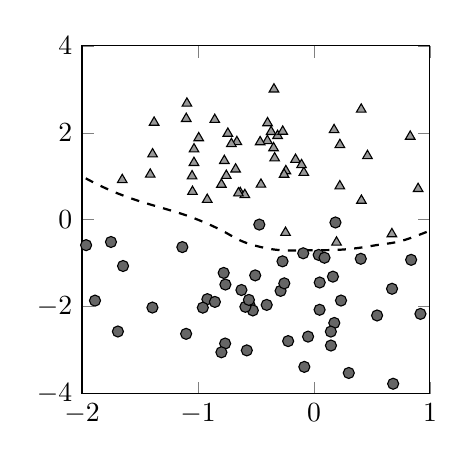
\begin{tikzpicture}
    \begin{axis}[
        width=6cm,height=6cm,
        ymin=-4,
        ymax=4,
        xmin=-2,
        xmax=1
    ]
        \draw[black, dashed, thick] plot[smooth,tension=0.75] coordinates
        {(-3, 3) (-2, 1) (-1, 0.0) (-0.5, -0.6) (0, -0.7) (0.5, -0.6) (1, -0.25) (2, 1)};
        \addplot[only marks,  mark size=2pt, draw=black, fill=black!40, mark=triangle*]
            table[x=x,y=y] {
                x           y
                -0.4017     1.8157
                -0.6757     1.1613
                -0.4004     2.2255
                -0.7981     0.811
                -0.1591     1.3838
                0.1945     -0.5193
                -1.3784     2.2377
                -0.4572     0.8124
                0.4091     0.442
                -0.7558     1.0147
                0.4613     1.4701
                -0.3138     1.9316
                -0.2454     -0.2958
                -1.1014     2.3242
                -1.6532     0.9184
                -1.0349     1.3118
                0.6718     -0.3262
                0.898     0.713
                -0.665     1.7912
                0.1733     2.0668
                -0.2426     1.1225
                -0.6358     0.6197
                -0.3451     3.0022
                0.2228     0.775
                -1.4119     1.0425
                1.2506     0.2047
                -1.0512     1.0045
                -0.3486     1.65
                -0.5962     0.5733
                -0.7428     1.9843
                -1.0344     1.624
                -1.3917     1.5095
                -0.2577     1.0401
                -0.6513     0.6118
                -0.9204     0.4636
                -1.0476     0.6458
                -0.7122     1.7462
                -1.0956     2.6759
                -0.3392     1.4172
                -0.8556     2.3016
                -0.3698     2.0229
                -0.4641     1.7882
                0.2234     1.7239
                -0.0875     1.0835
                -0.773     1.3568
                -0.1071     1.2615
                0.83     1.9156
                -0.2694     2.0301
                0.4074     2.5378
                -0.9939     1.8804
        };

        \addplot[only marks,  mark size=2pt, draw=black, fill=black!60,]
            table[x=x,y=y] {
                x           y
                -0.5566     -1.9559
                -0.0927     -0.7709
                -1.7505     -0.5113
                -0.0508     -2.6873
                0.1634     -1.3081
                -0.7786     -1.2223
                -1.6908     -2.5697
                -0.5271     -2.0852
                -1.965     -0.5841
                -0.0831     -3.3832
                -0.5915     -2.0022
                -0.2877     -1.6355
                0.1851     -0.0625
                -1.393     -2.0191
                -0.5791     -3.0039
                0.4037     -0.8977
                -0.2713     -0.9563
                -0.5612     -1.8431
                0.0403     -0.8086
                0.5443     -2.2012
                -0.9193     -1.8261
                0.0495     -1.4433
                0.1752     -2.3732
                -0.7661     -2.8464
                0.8378     -0.922
                -0.256     -1.4624
                -0.7982     -3.0478
                -0.2228     -2.7906
                0.0484     -2.07
                0.1463     -2.8925
                -2.2038     -1.8061
                -1.1024     -2.6235
                -0.7638     -1.4896
                -0.4713     -0.1112
                -0.6256     -1.6156
                0.3001     -3.5231
                -0.4076     -1.9581
                0.0908     -0.8736
                -1.6464     -1.0636
                0.6732     -1.5874
                0.9181     -2.1648
                -0.9585     -2.0214
                -2.3836     -1.9695
                -0.8543     -1.8891
                0.1455     -2.5717
                -1.8883     -1.8593
                -0.5068     -1.2795
                0.2331     -1.8579
                -1.135     -0.6287
                0.6828     -3.7712
        };

    \end{axis}
    \end{tikzpicture}%
        \caption{A poor fitted generative model: The original data (triangles) and the synthetic data (circles) can be easily separated by a classifier.}%
        \label{subfig:adversary_evaluation_bad}%
    \end{subfigure}%
    \hfill%
    \begin{subfigure}[b]{0.49\textwidth}%
        \centering\captionsetup{width=.8\linewidth}%
        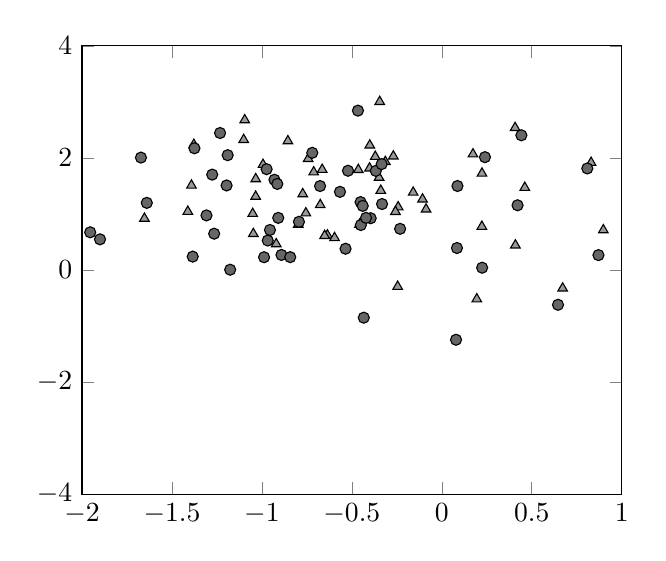
\begin{tikzpicture}

    \begin{axis}[
        ymin=-4,
        ymax=4,
        xmin=-2,
        xmax=1
    ]

        \addplot[only marks, draw=black, fill=black!40, mark=triangle*]
            table[x=x,y=y] {
                x           y
                -0.4017     1.8157
                -0.6757     1.1613
                -0.4004     2.2255
                -0.7981     0.811
                -0.1591     1.3838
                0.1945     -0.5193
                -1.3784     2.2377
                -0.4572     0.8124
                0.4091     0.442
                -0.7558     1.0147
                0.4613     1.4701
                -0.3138     1.9316
                -0.2454     -0.2958
                -1.1014     2.3242
                -1.6532     0.9184
                -1.0349     1.3118
                0.6718     -0.3262
                0.898     0.713
                -0.665     1.7912
                0.1733     2.0668
                -0.2426     1.1225
                -0.6358     0.6197
                -0.3451     3.0022
                0.2228     0.775
                -1.4119     1.0425
                1.2506     0.2047
                -1.0512     1.0045
                -0.3486     1.65
                -0.5962     0.5733
                -0.7428     1.9843
                -1.0344     1.624
                -1.3917     1.5095
                -0.2577     1.0401
                -0.6513     0.6118
                -0.9204     0.4636
                -1.0476     0.6458
                -0.7122     1.7462
                -1.0956     2.6759
                -0.3392     1.4172
                -0.8556     2.3016
                -0.3698     2.0229
                -0.4641     1.7882
                0.2234     1.7239
                -0.0875     1.0835
                -0.773     1.3568
                -0.1071     1.2615
                0.83     1.9156
                -0.2694     2.0301
                0.4074     2.5378
                -0.9939     1.8804
        };

        \addplot[only marks, draw=black, fill=black!60,]
            table[x=x,y=y] {
                x           y
                -0.5661     1.394
                -0.7942     0.8593
                -0.72     2.0904
                -0.9675     0.5258
                -0.3321     1.1766
                0.0791     -1.2452
                -1.6725     2.0054
                -0.535     0.3788
                0.2243     0.0403
                -0.9553     0.7138
                0.4212     1.1543
                -0.3669     1.7682
                -0.4338     -0.8514
                -1.3751     2.1716
                -1.9546     0.6723
                -1.3081     0.974
                0.646     -0.6215
                0.8709     0.2651
                -0.9304     1.6097
                0.2399     2.013
                -0.4501     0.8016
                -0.9881     0.2272
                -0.4661     2.8434
                0.0843     0.3917
                -1.9001     0.5467
                1.3748     -0.3017
                -1.2655     0.6477
                -0.4515     1.2111
                -0.8913     0.2683
                -0.9738     1.7986
                -1.1963     1.5083
                -1.64     1.1974
                -0.3954     0.9231
                -0.8426     0.2289
                -1.1765     0.0047
                -1.3847     0.2382
                -0.9144     1.5354
                -1.2327     2.444
                -0.4396     1.1434
                -1.1903     2.0482
                -0.3343     1.8891
                -0.6767     1.4974
                0.0871     1.4983
                -0.2318     0.734
                -0.9092     0.9296
                -0.4212     0.9299
                0.8089     1.8117
                -0.5214     1.7706
                0.4424     2.4034
                -1.2763     1.7014
        };

    \end{axis}
    \end{tikzpicture}%
        \caption{A well fitted generative model: The synthetic data resemble the original data well, such that a separation is not easy.}%
        \label{subfig:adversary_evaluation_good}%
    \end{subfigure}%
    \caption{Adversary evaluation: separation of original and synthetic data.}%
    \label{fig:adversary_evaluation}%
\end{figure}%
